\section{Importance of testing}
\setauthor{Romeo Bhuiyan}
The importance of testing cannot be overstated, particularly when it comes to 
assessing the user understanding and usability of the platform. Testing plays a crucial role in ensuring 
that Animotion is accessible and intuitive for a diverse range of users. By conducting testing, 
the Animotion-Team can gather valuable feedback from potential users, allowing them to identify 
potential pain points, areas of confusion, or any barriers that might hinder users from effectively getting 
the concept and using the platform seamlessly.

Testing the different functionalities involves engaging participants who represent the target audience and asking them to perform
specific tasks within the platform. Through these tests, the team can gain insights into how well users understand 
the Animotion concept, how easily they navigate through its features, and how efficiently they can accomplish desired 
actions. This process allows for the identification of any issues related to user comprehension, interface design, or 
interaction flow.

By analyzing the results of testing, designs can be improved for a better user experience. 
Adjustments can be made to enhance the clarity of instructions, improve visual cues, or streamline the workflow. Iterative 
testing and design modifications based on user feedback help to ensure that Animotion aligns with the expectations of the users, making 
it more user-friendly and approachable.

Incorporating accessibility testing is equally critical that Animotion is usable by individuals with diverse 
abilities. This involves testing the platform with individuals who have different cognitive, physical, and sensory abilities 
to identify potential accessibility challenges. Through this process, the Animotion developers can make necessary adjustments to ensure 
that Animotion is inclusive and can be accessed by all users, regardless of their capabilities.

\section{Theoretically applicable test methods}
\setauthor{Romeo Bhuiyan}

\subsection{Gathering information with a survey}
\setauthor{Romeo Bhuiyan}
Conducting testing through surveys is a valuable approach for Animotion to gain insights into user perceptions, 
preferences, and overall satisfaction. Surveys provide a structured way to collect feedback from a larger pool of users and 
can offer quantitative and qualitative data that informs design improvements.
A very important first step is to formulate a structured survey that covers a spectrum of usability factors. 
This includes the users initial impressions, simplicity of navigation, task completion and feature satisfaction.

There is also the possibility to gather information with demographic profiling, this can be useful for information such as 
age, occupation, familiarity with face and body tracking tools, and virtual reality technologies which provides context for interpreting the data correctly.
This profiling helps in identifying patterns and preferences across different user segments.
In terms of feature satisfaction a Likert scales or rating system can be incorporated to measure these data.
This data allows for easy statistical analysis, revealing trends and patterns that can be used again to for example implement a new VRM model or improve other features.
Open-ended questions with a free space to type in or comment sections enable users to provide detailed qualitative feedback.
These can be used for ideas or specific problems that users encountered, also not covered questions in the survey can be pointed out there. \cite{syp}

Using surveys as a method for testing offers a multitude of benefits that contribute to the comprehensive assessment of user experiences and perceptions. 
These advantages make surveys a valuable tool for Animotion in understanding how users interact with their application and identifying areas for improvement.
One of them is their scalability which can be effortlessly distributed to a large number of users simultaneously. 
This makes them an efficient choice for collecting data from a diverse and extensive user base. 
Money is also a very improtant factor to keep in mind so the cost-effectiveness of surveys is a big plus. 

Traditional approaches like in-person interviews or observations often entail higher 
costs related to logistics and resources. On the other hand, designing, distributing, and collecting responses from surveys can be 
achieved with minimal financial investment. Extracting the data is also very easy due to the structured nature of surveys.
This structured format enables Animotion to extract valuable statistical insights and identify trends from the useres point of view.
This data-driven approach provides a clear understanding of the prevalence of specific usability issues and helps prioritize improvements.
All also participants receive the same set of questions, minimizing variations caused by misinterpretations. 
This consistency enhances the reliability and accuracy of the data gathered.

Questionaieres also have a few limitations that Animotion should be aware of when using them as a testing method.
They may not uncover the depth of user experiences, as they lack the ability to capture underlying reasons behind responses. 
Responses can also be influenced by subjective bias, potentially skewing the results.
To address these limitations, Animotion can consider combining surveys with other methods like user observations, interviews, 
or usability testing. This multi-faceted approach can provide a more comprehensive understanding of user experiences and 
ensure a well-rounded evaluation of usability. \cite{questionaire}

\subsection{Having a conversation in an interview}
\setauthor{Romeo Bhuiyan}
Using the interview method offers Animotion a rich avenue for gathering valuable insights into users' 
experiences, thoughts, and perceptions. Interviews provide an opportunity to engage with participants in a more 
personalized and interactive manner, allowing for in-depth exploration of their behaviors, motivations and challenges when using Animotion's platform.
Through interviews, Animotion can delve into users' thought processes and uncover the reasons behind their interactions with the platform. 
This method allows participants to express their opinions and provide context that might not be captured through quantitative data alone.
Participants can describe their experiences in their own words, offering unique perspectives that quantitative measures might miss. 
This qualitative data can be particularly valuable in identifying nuanced issues, understanding user emotions, and uncovering 
unexpected trends. \cite{syp}

A beneficial feature of intereviews is that Animotion can also observe users' facial expressions, gestures, and body 
language, providing additional non-verbal cues that shed light on their feelings and reactions. This approach allows 
for a more comprehensive evaluation of the user experience. There are also many downsides of this method as the time-consumption
because  each interview requires careful planning, execution, and analysis. Interviewing also demands strong interpersonal skills to 
establish rapport with participants and create an environment where they feel comfortable sharing their thoughts. \cite{interview}

\subsection{Following the user with eye tracking}
\setauthor{Romeo Bhuiyan}
Integrating eye tracking technology into usability testing represents a cutting-edge approach for Animotion to gain profound insights into users'
interactions with the platform. This method involves the use of specialized hardware and software to precisely monitor participants' eye movements,
gaze points and fixations as they navigate Animotion's interface and use the application. This technology allows for the identification of which areas 
of the platform draw the most attention, helping to ascertain the effectiveness of design elements, layout, and content placement. 
Animotion can determine whether key features or information are being overlooked, pinpointing potential usability issues.
It also enables the measurement of the time users spend on specific interface elements. This data can reveal the efficiency of interactions,
indicating whether users quickly find what they need or if they struggle with navigation. Animotion can identify bottlenecks and 
areas where users might get stuck, informing targeted improvements. \cite{eye1}

To work with that approach it is clever to combine eye tracking with other methods like surveys or interviews to gain a more comprehensive understanding of users
cognitive processes and emotional responses. Animotion can determine what users are thinking and feeling as they interact with the platform, 
uncovering pain points and areas of satisfaction. There are also some difficulties to consider when employing eye tracking technology. 
The equipment can be expensive and requires skilled setup and calibration to ensure accurate data collection. Privacy concerns might 
also arise, as tracking users' gaze points raises ethical considerations regarding data protection. \cite{eye2}

\section{Target Groups}
\setauthor{Romeo Bhuiyan}
Animotion can reach a diverse array of target groups, each finding value in its fusion of AI-driven technologies 
and 3D animation. It is designed to be with both professional and amateurs users, Animotion findes relevance in multiple fields
offering tailored benefits to various segments.
At the core of Animotion's target audience are Content creators, including YouTubers and social media influencers, 
can elevate their content with Animotion. The integration of 3D avatars and animations enhances visual appeal 
and engagement, providing creators with tools to create dynamic and captivating content as seen in the paragraph below.
The entertainment industry has also embraced face and body tracking technology, using it to create more engaging and 
interactive experiences for audiences. The technology can be used to track the movements and expressions of performers, 
allowing them to control animated characters or special effects in real-time. For example, the Cirque du Soleil show "KÀ" uses face and body 
tracking technology to create a seamless blend of live performance and digital effects, enhancing the audience's experience. \cite{cirque}

There is also the use of Animotion for dancers and prefromers where this dynamic interaction between the dancer and the 
virtual avatar opens doors for innovation and experimentation, fostering the evolution of artistic expressions. A significant aspect 
is Animotion's capacity to empower even shy individuals to express their artistry with confidence. For those who might feel hesitant 
or self-conscious in front of an audience, Animotion provides a safe and private space to explore their creativity. By embodying 
their art through avatars, dancers can detach from personal inhibitions and fully immerse themselves in their craft. 
This unique feature offers a liberating experience, where emotions and artistic visions can be channeled without the constraints of self-consciousness.
Experienced dancers can also record their performance to aspire newcomers to explore the world of dancing, this also leads to an engaging and interactive manner.
They can receive guidance from experts without the pressure of a traditional classroom setting and embark on their dance journey with confidence and enthusiasm.

Animotion holds immense potential for the game development industry, introducing a dynamic and interactive element that enhances user engagement and realism. Especially 
in terms of fitness. This offer a new dimension to staying active and healthy. These games utilize users' real-world movements to control 
in-game actions, making workouts engaging and enjoyable. From dance routines that sync with players' motions to virtual sports that encourage 
physical activity, fitness games merge gaming with exercise, encouraging players to break a sweat while having fun. Animotion's technology 
transforms the usual webcam on a generic pc into a fitness tool, promoting a healthier lifestyle through interactive and entertaining gameplay.

\subsection{Virtual Youtubers as a trend}
\setauthor{Romeo Bhuiyan}
Virtual YouTubers or also called VTubers are online content creators who use virtual avatars or characters to engage with their 
audience on platforms like YouTube and Twitch. These avatars are brought to life through animation, motion capture, 
or AI technologies, allowing the creators to interact with viewers in a more immersive and entertaining way. 
VTubers often stream gameplay, discussions, and live performances, attracting audiences who appreciate the 
unique blend of personality and digital artistry. VTubers have gained lots of popularity over time as shown in the graph \ref{fig:vtubers} below.
The appeal of VTubers lies in their ability to transcend cultural and linguistic barriers. As digital avatars, 
VTubers can represent a wide range of characters and identities, appealing to diverse audiences worldwide. 
This inclusivity and adaptability contribute to their widespread popularity. \cite{vtubing1}
\\
\begin{figure}[htb]
    \centering
    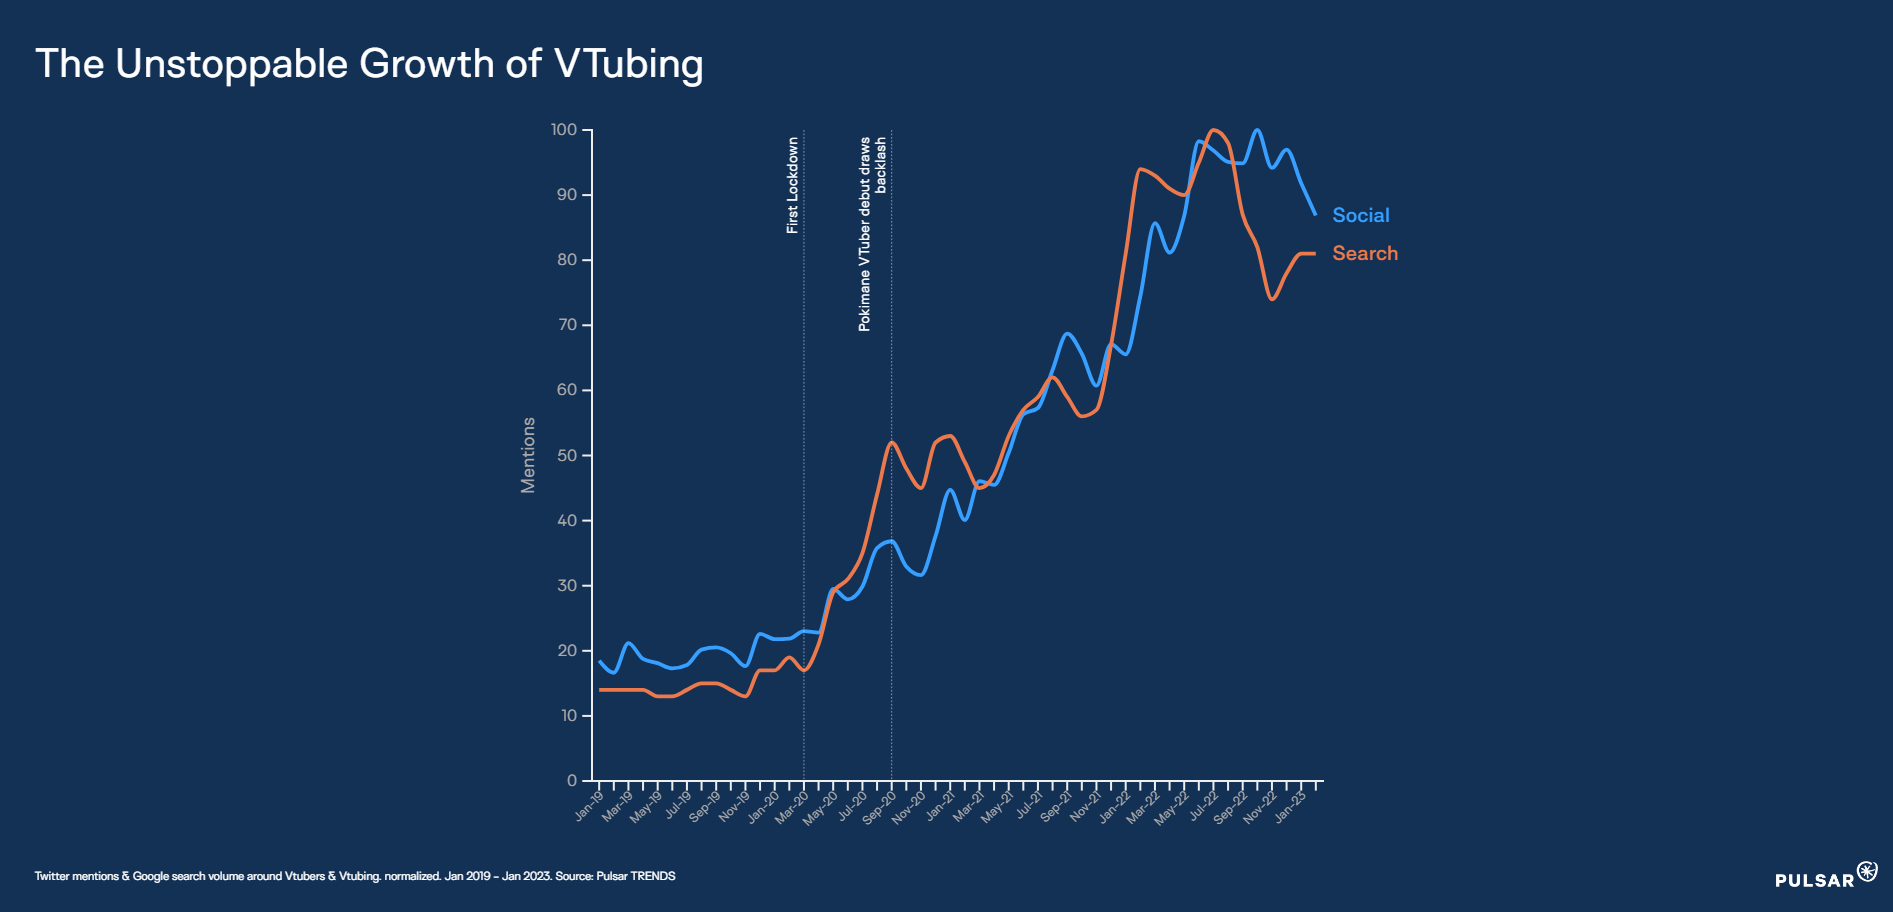
\includegraphics[width=0.9\textwidth]{pics/riseofvtubers.png}
    \caption{Popularity of VTubing shown from January in 2019 till January in 2023}
    \cite{vtubing1}
    \label{fig:vtubers}
\end{figure}
\\
The younger generation, often referred to as \emph{Gen Z,} has embraced VTubers due to their affinity for digital content and online interactions. 
VTubers offer an engaging and relatable form of entertainment that aligns with the nature of Gen Z. The interactive nature of live streams and the 
sense of direct connection with VTubers foster a strong sense of community, making fans feel like 
active participants rather than passive consumers.
VTubers have also capitalized on trends in social media and content creation. Platforms like YouTube, Twitch, 
and other live-streaming services have played a pivotal role in the VTuber phenomenon. In particular, the \emph{Just Chatting} section on Twitch has become 
a hotspot for VTubers, allowing them to engage in conversations, share experiences, and showcase their unique personalities beyond gaming. \cite{vtubing2}

The \emph{Just Chatting} section on Twitch has gained immense popularity as seen in the figure \ref{fig:justchattwitch} below, by providing a space for 
streamers to engage with their viewers through casual conversations, discussions, and activities. Many VTubers have found success in this category, as 
it allows them to showcase their avatars and personalities while interacting directly with fans. The section's growth signifies the audience's 
interest in more intimate and personal content, where content creators can share stories, opinions, and experiences, fostering a strong sense of community and connection.
\\
\begin{figure}[htb]
    \centering
    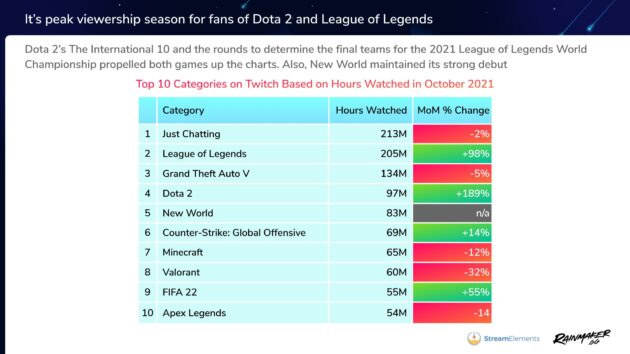
\includegraphics[width=0.9\textwidth]{pics/justchattwitch.jpg}
    \caption{Popularity of different Twitch categories 2021}
    \cite{geekwire}
    \label{fig:justchattwitch}
\end{figure}
\\
\section{Test Report}
\setauthor{Romeo Bhuiyan}
The purpose of this report is to provide a comprehensive analysis of the usability testing of Animotion, a web application that uses face and 
body tracking technology. The Animotion test, conducted with the participation of 116 individuals from Tadeot at the 
HTL Leonding for a comprehensive analysis of user interactions, impressions, and insights, shedding light on how Animotion's 
fusion of AI, motion tracking, and creative expression resonates with the participants. 
The report will discuss the results of the testing and provide recommendations for future improvements.

\subsection{Setting in which the test took place}
\setauthor{Romeo Bhuiyan}
The usability testing was conducted with a total of 116 participants, consisting of 84 people aged between 12 and 15 years old with little experience 
with information technology and artificial intelligence, three people over 30 years old with some experience in these areas, and 29 people 
between 16 and 30 years old with high experience. Participants were selected from the Tadeot of the HTL Leonding in Austria. 
The testing was conducted in a controlled environment with participants seated in front of a computer screen.
The participants, who were standing in front of a computer screen, received a short explanation of Animotion's functionality. 
Following this, they were tasked with using the web application to monitor their facial and body movements. 
The participants were asked what they thought about how easy the app was to use, how well it tracked their movements, and if they had any problems using it.

\subsection{Result}
\setauthor{Romeo Bhuiyan}
The results of the usability testing were generally positive. Of the self-evaluated data, 95.14 \% of participants were able to intuitively 
understand what the application did without needing an explanation. This indicates that Animotion is user-friendly and easy to understand for most users.
Nevertheless, during the testing phase, certain limitations in Animotion's performance became evident. Notably, participants encountered challenges with the 
application's ability to accurately track facial and bodily motions. A subset of users reported instances where the tracking precision did not meet their 
expectations, leading to difficulties in achieving the desired responsiveness from the application.
The participants also identified a couple of noteworthy shortcomings. One particular issue pertains to the application's inability to 
display the VRM model when the user's back is turned to the camera and no facial features are detected. In addition to that, users noticed that if they 
turned to a specific degree, the AI's tracking capabilities became impaired, resulting in an interruption in smooth tracking.

\subsection{Conclusion}
\setauthor{Romoe Bhuiyan}   
In conclusion, the comprehensive testing of Animotion has revealed the web application's overall effectiveness and user-friendly design. 
There were some worries about how accurate the tracking is and how easy the app is to use. To make the app even better, 
the team can focus on fixing these things by listening to users and making improvements based on their feedback. 
This will make Animotion more user-friendly and enjoyable for everyone.
